% Options for packages loaded elsewhere
\PassOptionsToPackage{unicode}{hyperref}
\PassOptionsToPackage{hyphens}{url}
\PassOptionsToPackage{dvipsnames,svgnames,x11names}{xcolor}
%
\documentclass[
  letterpaper,
  DIV=11,
  numbers=noendperiod]{scrreprt}

\usepackage{amsmath,amssymb}
\usepackage{iftex}
\ifPDFTeX
  \usepackage[T1]{fontenc}
  \usepackage[utf8]{inputenc}
  \usepackage{textcomp} % provide euro and other symbols
\else % if luatex or xetex
  \usepackage{unicode-math}
  \defaultfontfeatures{Scale=MatchLowercase}
  \defaultfontfeatures[\rmfamily]{Ligatures=TeX,Scale=1}
\fi
\usepackage{lmodern}
\ifPDFTeX\else  
    % xetex/luatex font selection
\fi
% Use upquote if available, for straight quotes in verbatim environments
\IfFileExists{upquote.sty}{\usepackage{upquote}}{}
\IfFileExists{microtype.sty}{% use microtype if available
  \usepackage[]{microtype}
  \UseMicrotypeSet[protrusion]{basicmath} % disable protrusion for tt fonts
}{}
\makeatletter
\@ifundefined{KOMAClassName}{% if non-KOMA class
  \IfFileExists{parskip.sty}{%
    \usepackage{parskip}
  }{% else
    \setlength{\parindent}{0pt}
    \setlength{\parskip}{6pt plus 2pt minus 1pt}}
}{% if KOMA class
  \KOMAoptions{parskip=half}}
\makeatother
\usepackage{xcolor}
\setlength{\emergencystretch}{3em} % prevent overfull lines
\setcounter{secnumdepth}{5}
% Make \paragraph and \subparagraph free-standing
\ifx\paragraph\undefined\else
  \let\oldparagraph\paragraph
  \renewcommand{\paragraph}[1]{\oldparagraph{#1}\mbox{}}
\fi
\ifx\subparagraph\undefined\else
  \let\oldsubparagraph\subparagraph
  \renewcommand{\subparagraph}[1]{\oldsubparagraph{#1}\mbox{}}
\fi

\usepackage{color}
\usepackage{fancyvrb}
\newcommand{\VerbBar}{|}
\newcommand{\VERB}{\Verb[commandchars=\\\{\}]}
\DefineVerbatimEnvironment{Highlighting}{Verbatim}{commandchars=\\\{\}}
% Add ',fontsize=\small' for more characters per line
\usepackage{framed}
\definecolor{shadecolor}{RGB}{241,243,245}
\newenvironment{Shaded}{\begin{snugshade}}{\end{snugshade}}
\newcommand{\AlertTok}[1]{\textcolor[rgb]{0.68,0.00,0.00}{#1}}
\newcommand{\AnnotationTok}[1]{\textcolor[rgb]{0.37,0.37,0.37}{#1}}
\newcommand{\AttributeTok}[1]{\textcolor[rgb]{0.40,0.45,0.13}{#1}}
\newcommand{\BaseNTok}[1]{\textcolor[rgb]{0.68,0.00,0.00}{#1}}
\newcommand{\BuiltInTok}[1]{\textcolor[rgb]{0.00,0.23,0.31}{#1}}
\newcommand{\CharTok}[1]{\textcolor[rgb]{0.13,0.47,0.30}{#1}}
\newcommand{\CommentTok}[1]{\textcolor[rgb]{0.37,0.37,0.37}{#1}}
\newcommand{\CommentVarTok}[1]{\textcolor[rgb]{0.37,0.37,0.37}{\textit{#1}}}
\newcommand{\ConstantTok}[1]{\textcolor[rgb]{0.56,0.35,0.01}{#1}}
\newcommand{\ControlFlowTok}[1]{\textcolor[rgb]{0.00,0.23,0.31}{#1}}
\newcommand{\DataTypeTok}[1]{\textcolor[rgb]{0.68,0.00,0.00}{#1}}
\newcommand{\DecValTok}[1]{\textcolor[rgb]{0.68,0.00,0.00}{#1}}
\newcommand{\DocumentationTok}[1]{\textcolor[rgb]{0.37,0.37,0.37}{\textit{#1}}}
\newcommand{\ErrorTok}[1]{\textcolor[rgb]{0.68,0.00,0.00}{#1}}
\newcommand{\ExtensionTok}[1]{\textcolor[rgb]{0.00,0.23,0.31}{#1}}
\newcommand{\FloatTok}[1]{\textcolor[rgb]{0.68,0.00,0.00}{#1}}
\newcommand{\FunctionTok}[1]{\textcolor[rgb]{0.28,0.35,0.67}{#1}}
\newcommand{\ImportTok}[1]{\textcolor[rgb]{0.00,0.46,0.62}{#1}}
\newcommand{\InformationTok}[1]{\textcolor[rgb]{0.37,0.37,0.37}{#1}}
\newcommand{\KeywordTok}[1]{\textcolor[rgb]{0.00,0.23,0.31}{#1}}
\newcommand{\NormalTok}[1]{\textcolor[rgb]{0.00,0.23,0.31}{#1}}
\newcommand{\OperatorTok}[1]{\textcolor[rgb]{0.37,0.37,0.37}{#1}}
\newcommand{\OtherTok}[1]{\textcolor[rgb]{0.00,0.23,0.31}{#1}}
\newcommand{\PreprocessorTok}[1]{\textcolor[rgb]{0.68,0.00,0.00}{#1}}
\newcommand{\RegionMarkerTok}[1]{\textcolor[rgb]{0.00,0.23,0.31}{#1}}
\newcommand{\SpecialCharTok}[1]{\textcolor[rgb]{0.37,0.37,0.37}{#1}}
\newcommand{\SpecialStringTok}[1]{\textcolor[rgb]{0.13,0.47,0.30}{#1}}
\newcommand{\StringTok}[1]{\textcolor[rgb]{0.13,0.47,0.30}{#1}}
\newcommand{\VariableTok}[1]{\textcolor[rgb]{0.07,0.07,0.07}{#1}}
\newcommand{\VerbatimStringTok}[1]{\textcolor[rgb]{0.13,0.47,0.30}{#1}}
\newcommand{\WarningTok}[1]{\textcolor[rgb]{0.37,0.37,0.37}{\textit{#1}}}

\providecommand{\tightlist}{%
  \setlength{\itemsep}{0pt}\setlength{\parskip}{0pt}}\usepackage{longtable,booktabs,array}
\usepackage{calc} % for calculating minipage widths
% Correct order of tables after \paragraph or \subparagraph
\usepackage{etoolbox}
\makeatletter
\patchcmd\longtable{\par}{\if@noskipsec\mbox{}\fi\par}{}{}
\makeatother
% Allow footnotes in longtable head/foot
\IfFileExists{footnotehyper.sty}{\usepackage{footnotehyper}}{\usepackage{footnote}}
\makesavenoteenv{longtable}
\usepackage{graphicx}
\makeatletter
\def\maxwidth{\ifdim\Gin@nat@width>\linewidth\linewidth\else\Gin@nat@width\fi}
\def\maxheight{\ifdim\Gin@nat@height>\textheight\textheight\else\Gin@nat@height\fi}
\makeatother
% Scale images if necessary, so that they will not overflow the page
% margins by default, and it is still possible to overwrite the defaults
% using explicit options in \includegraphics[width, height, ...]{}
\setkeys{Gin}{width=\maxwidth,height=\maxheight,keepaspectratio}
% Set default figure placement to htbp
\makeatletter
\def\fps@figure{htbp}
\makeatother
% definitions for citeproc citations
\NewDocumentCommand\citeproctext{}{}
\NewDocumentCommand\citeproc{mm}{%
  \begingroup\def\citeproctext{#2}\cite{#1}\endgroup}
\makeatletter
 % allow citations to break across lines
 \let\@cite@ofmt\@firstofone
 % avoid brackets around text for \cite:
 \def\@biblabel#1{}
 \def\@cite#1#2{{#1\if@tempswa , #2\fi}}
\makeatother
\newlength{\cslhangindent}
\setlength{\cslhangindent}{1.5em}
\newlength{\csllabelwidth}
\setlength{\csllabelwidth}{3em}
\newenvironment{CSLReferences}[2] % #1 hanging-indent, #2 entry-spacing
 {\begin{list}{}{%
  \setlength{\itemindent}{0pt}
  \setlength{\leftmargin}{0pt}
  \setlength{\parsep}{0pt}
  % turn on hanging indent if param 1 is 1
  \ifodd #1
   \setlength{\leftmargin}{\cslhangindent}
   \setlength{\itemindent}{-1\cslhangindent}
  \fi
  % set entry spacing
  \setlength{\itemsep}{#2\baselineskip}}}
 {\end{list}}
\usepackage{calc}
\newcommand{\CSLBlock}[1]{\hfill\break\parbox[t]{\linewidth}{\strut\ignorespaces#1\strut}}
\newcommand{\CSLLeftMargin}[1]{\parbox[t]{\csllabelwidth}{\strut#1\strut}}
\newcommand{\CSLRightInline}[1]{\parbox[t]{\linewidth - \csllabelwidth}{\strut#1\strut}}
\newcommand{\CSLIndent}[1]{\hspace{\cslhangindent}#1}

\usepackage{booktabs}
\usepackage{caption}
\usepackage{longtable}
\usepackage{colortbl}
\usepackage{array}
\usepackage{anyfontsize}
\usepackage{multirow}
\KOMAoption{captions}{tableheading}
\makeatletter
\@ifpackageloaded{bookmark}{}{\usepackage{bookmark}}
\makeatother
\makeatletter
\@ifpackageloaded{caption}{}{\usepackage{caption}}
\AtBeginDocument{%
\ifdefined\contentsname
  \renewcommand*\contentsname{Table of contents}
\else
  \newcommand\contentsname{Table of contents}
\fi
\ifdefined\listfigurename
  \renewcommand*\listfigurename{List of Figures}
\else
  \newcommand\listfigurename{List of Figures}
\fi
\ifdefined\listtablename
  \renewcommand*\listtablename{List of Tables}
\else
  \newcommand\listtablename{List of Tables}
\fi
\ifdefined\figurename
  \renewcommand*\figurename{Figure}
\else
  \newcommand\figurename{Figure}
\fi
\ifdefined\tablename
  \renewcommand*\tablename{Table}
\else
  \newcommand\tablename{Table}
\fi
}
\@ifpackageloaded{float}{}{\usepackage{float}}
\floatstyle{ruled}
\@ifundefined{c@chapter}{\newfloat{codelisting}{h}{lop}}{\newfloat{codelisting}{h}{lop}[chapter]}
\floatname{codelisting}{Listing}
\newcommand*\listoflistings{\listof{codelisting}{List of Listings}}
\usepackage{amsthm}
\theoremstyle{definition}
\newtheorem{exercise}{Exercise}[chapter]
\theoremstyle{remark}
\AtBeginDocument{\renewcommand*{\proofname}{Proof}}
\newtheorem*{remark}{Remark}
\newtheorem*{solution}{Solution}
\newtheorem{refremark}{Remark}[chapter]
\newtheorem{refsolution}{Solution}[chapter]
\makeatother
\makeatletter
\makeatother
\makeatletter
\@ifpackageloaded{caption}{}{\usepackage{caption}}
\@ifpackageloaded{subcaption}{}{\usepackage{subcaption}}
\makeatother
\ifLuaTeX
  \usepackage{selnolig}  % disable illegal ligatures
\fi
\usepackage{bookmark}

\IfFileExists{xurl.sty}{\usepackage{xurl}}{} % add URL line breaks if available
\urlstyle{same} % disable monospaced font for URLs
\hypersetup{
  pdfauthor={SDIV},
  colorlinks=true,
  linkcolor={blue},
  filecolor={Maroon},
  citecolor={Blue},
  urlcolor={Blue},
  pdfcreator={LaTeX via pandoc}}

\author{Saúl Díaz Infante, David González Sánchez}
\date{2024-05-30}

\begin{document}

\renewcommand*\contentsname{Table of contents}
{
\hypersetup{linkcolor=}
\setcounter{tocdepth}{2}
\tableofcontents
}
\bookmarksetup{startatroot}

\chapter*{Preface}\label{preface}
\addcontentsline{toc}{chapter}{Preface}

\markboth{Preface}{Preface}

This notes are based in the course from Berstekas for the MIT see all
lectures and other resources for complete the understanding.

\section*{Abstract}\label{abstract}
\addcontentsline{toc}{section}{Abstract}

\markright{Abstract}

We present an introduction to the solution of multi-stage optimization
problems. Starting from the dynamic programming algorithm, we consider
theoretical and computational aspects, mainly of deterministic problems,
and discuss how to generalize some of the results to Markovian decision
processes.

The classic problem with which the essential ideas of dynamic
programming can be introduced is the optimal route problem (shortest
route considering distances, or cheapest route considering costs)
(Bertsekas 2005; Brandimarte 2013). A simple version of this problem is
shown schematically in Fig~\ref{fig-brandimarte_net}. By exhaustion, we
deploy the cost of path in Table~\ref{tbl-brandimarte_paths}.

\begin{figure}

\centering{

\includegraphics{../assets/ch_00/network_brandimarte_ex.png}

}

\caption{\label{fig-brandimarte_net}The shortest path}

\end{figure}%

\begin{longtable}[]{@{}lc@{}}
\caption{The shortest path by exhaustion see (Brandimarte
2013).}\label{tbl-brandimarte_paths}\tabularnewline
\toprule\noalign{}
Path & Cost \\
\midrule\noalign{}
\endfirsthead
\toprule\noalign{}
Path & Cost \\
\midrule\noalign{}
\endhead
\bottomrule\noalign{}
\endlastfoot
\(0 \to 1 \to 4 \to 7\) & 18 \\
\(0 \to 1 \to 3 \to 4 \to 7\) & 22 \\
\(0 \to 1 \to 3 \to 6 \to 7\) & 18 \\
\(0 \to 1 \to 3 \to 5 \to 6 \to 7\) & 20 \\
\(\mathbf{0 \to 1 \to 3 \to 5 \to 7}\) & \textbf{16} \\
\(0 \to 2 \to 3 \to 4 \to 7\) & 23 \\
\(0 \to 2 \to 3 \to 6 \to 7\) & 19 \\
\(0 \to 2 \to 3 \to 5 \to 6 \to 7\) & 21 \\
\(0 \to 2 \to 3 \to 5 \to 7\) & 17 \\
\(0 \to 2 \to 5 \to 6 \to 7\) & 22 \\
\(0 \to 2 \to 5 \to 7\) & 18 \\
\end{longtable}

In this problem, the optimal route to go from the node labeled \(0\) to
the node labeled \(7\) is to be determined. The costs between each pair
of nodes connected by an arrow are represented by a number next to it.
For example, the cost to go from node 0 to node 2 is 6. The optimal
route will be the one for which the sum of their costs is minimum. This
optimal route can be obtained by an exhaustive enumeration; generating
all possible routes from node \(0\) to node \(7\) and choosing the
minimum cost route.

En la {[}ref:table{]} se muestran tales rutas y sus respectivos costos.
Se observa que la trayectoria óptima es \$ 0 \to   1 \to 3 \to 5 \to  7
\$, con un costo de 16.

\bookmarksetup{startatroot}

\chapter*{Outline}\label{outline}
\addcontentsline{toc}{chapter}{Outline}

\markboth{Outline}{Outline}

The textbook for chapter one is Bertsekas' book (Bertsekas 2005).
Chapters 2 and 3 are adapted from Sutton's book (Ch. 3, Ch. 4, Sutton
and Barto 2018). For application and broad connection with more machine
learning applications, we refer to (Brunton and Kutz 2019). Also, we
recommend a handbook of algorithms (Szepesvári 2022). For applications
with implemented code, we follow the books (Bilgin 2020).

\bookmarksetup{startatroot}

\chapter*{Abstract}\label{abstract-1}
\addcontentsline{toc}{chapter}{Abstract}

\markboth{Abstract}{Abstract}

We present an introduction to the solution of multi-stage optimization
problems. Starting from the dynamic programming algorithm, we consider
theoretical and computational aspects, mainly of deterministic problems,
and discuss how to generalize some of the results to Markovian decision
processes.

The classic problem with which the essential ideas of dynamic
programming can be introduced is the optimal route problem (shortest
route considering distances, or cheapest route considering costs)
(Bertsekas 2005; Brandimarte 2013). A simple version of this problem is
shown schematically in Fig~\ref{fig-brandimarte_net}. By exhaustion, we
deploy the cost of path in Table~\ref{tbl-brandimarte_paths}.

\begin{figure}

\centering{

\includegraphics{01-introduction/../assets/ch_00/network_brandimarte_ex.png}

}

\caption{\label{fig-brandimarte_net}The shortest path}

\end{figure}%

\begin{longtable}[]{@{}lc@{}}
\caption{The shortest path by exhaustion see (Brandimarte
2013).}\label{tbl-brandimarte_paths}\tabularnewline
\toprule\noalign{}
Path & Cost \\
\midrule\noalign{}
\endfirsthead
\toprule\noalign{}
Path & Cost \\
\midrule\noalign{}
\endhead
\bottomrule\noalign{}
\endlastfoot
\(0 \to 1 \to 4 \to 7\) & 18 \\
\(0 \to 1 \to 3 \to 4 \to 7\) & 22 \\
\(0 \to 1 \to 3 \to 6 \to 7\) & 18 \\
\(0 \to 1 \to 3 \to 5 \to 6 \to 7\) & 20 \\
\(\mathbf{0 \to 1 \to 3 \to 5 \to 7}\) & \textbf{16} \\
\(0 \to 2 \to 3 \to 4 \to 7\) & 23 \\
\(0 \to 2 \to 3 \to 6 \to 7\) & 19 \\
\(0 \to 2 \to 3 \to 5 \to 6 \to 7\) & 21 \\
\(0 \to 2 \to 3 \to 5 \to 7\) & 17 \\
\(0 \to 2 \to 5 \to 6 \to 7\) & 22 \\
\(0 \to 2 \to 5 \to 7\) & 18 \\
\end{longtable}

In this problem, the optimal route to go from the node labeled \(0\) to
the node labeled \(7\) is to be determined. The costs between each pair
of nodes connected by an arrow are represented by a number next to it.
For example, the cost to go from node 0 to node 2 is 6. The optimal
route will be the one for which the sum of their costs is minimum. This
optimal route can be obtained by an exhaustive enumeration; generating
all possible routes from node \(0\) to node \(7\) and choosing the
minimum cost route.

En la {[}ref:table{]} se muestran tales rutas y sus respectivos costos.
Se observa que la trayectoria óptima es \$ 0 \to   1 \to 3 \to 5 \to  7
\$, con un costo de 16.

\bookmarksetup{startatroot}

\chapter{Introduction}\label{introduction}

Reinforcement Learning is part of a decades-long trend within artificial
intelligence and machine learning toward greater integration with
statistics, optimization, and other mathematical subjects. For example,
the ability of some reinforcement learning methods to learn with
parameterized approximators addresses the classical ``curse of
dimensionality'' in operations research and control theory. More
distinctively, reinforcement learning has also interacted strongly with
psychology and neuroscience, with substantial benefits going both ways.
Of all the forms of machine learning, reinforcement learning is the
closest to the kind of learning that humans and other animals do, and
many of the core algorithms of reinforcement learning were originally
inspired by biological learning systems.

\section{Trial-Error}\label{trial-error}

According to Richard S. Sutton and Andrew G. Barto Sutton and Barto
(2018)--the first authors to use the term--Reinforced Learning
Reinforcement learning is about what to do, that is, how to map
situations to action so that we optimize a reward. \textbf{The learner
must discover which action yield the best reward by trying them.} In the
most general sense, action may not only affect immediate reward but also
the next situation and, through that, all subsequent rewards.

\subsection{Sensation action and goal}\label{sensation-action-and-goal}

At the same time, Reinforcement Learning encloses a problem, a class of
solution methods, and the field that studies this problem and its
solutions. Its formalism is based on the theory of controlled dynamical
systems, with a strong focus on the optimal control of partially known
Markov decision processes. Then, the core idea consists of capturing the
essence of the problem when an agent learns through experience and
interaction to reach a goal. This agent can sense the state of its
environment to some extent and must be able to take action that affects
the state. The agent also must have a goal or goals related to the state
of the environment.

MDPs are designed to incorporate three essential elements: sensation,
action, and goal. Therefore, any approach suitable for solving such
problems should be considered a potential method for Reinforcement
Learning.

\section{Exploration-exploration dilemma and
uncertainty}\label{exploration-exploration-dilemma-and-uncertainty}

To obtain the best reward, the agent must prefer actions used in the
past and perceived as effective to produce a reward. However, to
discover such actions, the agent must try actions never used before. So,
there is a delicate trade-off between exploiting and exploring. The
agent has to exploit its knowledge to produce a reward but
simultaneously has to explore to improve its reward in the future. Here,
our dilemma is that neither exploration nor exploitation can be pursued
exclusively without failing the task.

Another essential aspect of reinforcement learning is that it
specifically deals with the entire process of a goal-directed agent
interacting with an uncertain environment. This aspect differs from many
approaches that only focus on subproblems rather than considering how
they might contribute to the bigger picture. For example, many machine
learning researchers have studied supervised Learning without specifying
how such an ability would ultimately be helpful. Other researchers have
developed planning theories with general goals without considering
planning's role in real-time decision-making or whether the predictive
models necessary for planning are well suited. Although these approaches
have produced valuable results, their focus on isolated subproblems
leads to significant limitations.

Reinforcement learning takes the opposite approach, beginning with a
fully interactive, goal-seeking agent. In reinforcement learning, the
agent has explicit goals, can sense aspects of their environment, and
can choose actions to influence its environment.

\section{Examples}\label{examples}

\begin{itemize}
\item
  A master chess player makes a move.
\item
  An adaptive controller adjusts parameters of a petroleum refinery's
  operation in real time.
\item
  A gazelle calf struggles to its feet minutes after being born.
\item
  A mobile robot decides whether it should enter a new room in search of
  more trash to collect or start trying to find its way back to its
  battery recharging station.
\item
  Phil prepares his breakfast
\end{itemize}

\section{The (possible) 4 elements of Reinforcement
Learning}\label{the-possible-4-elements-of-reinforcement-learning}

Given an agent, we identify four main element in a reinforcement
learning model:

\begin{quote}
a \textbf{policy}, a \textbf{reward}, a value function and (optionally)
a model of the \textbf{environment}.
\end{quote}

\begin{description}
\item[Policy]
A policy is as a set of actions that guide the agent to respond
according to its perception of the environment. It's like a set of
instructions that tell the agent what to do when it encounters a certain
situation. In general, policies may be stochastic, specifying
probabilities for each action.
\item[Reward]
The reward signal thus defines what are the good and bad events for the
agent. In a biological system, we might think of rewards as analogous to
the experiences of pleasure or pain. They are the immediate and defining
features of the problem faced by the agent. The reward signal is the
primary basis for altering the policy; if an action selected by the
policy is followed by low reward, then the policy may be changed to
select some other action in that situation in the future. In general,
reward signals may be stochastic functions of the state of the
environment and the actions taken.
\item[Value function]
Whereas the reward signal indicates what is good in the immediate sense,
a value function specifies what is good in the long run. In simple
terms, the value of a state represents the total reward an agent can
anticipate to receive in the future, beginning from that state. While
rewards reflect the immediate appeal of environmental states, values
signify the long-term appeal of states, considering the potential future
states and the rewards they offer. For example, a state might
consistently yield a low immediate reward but still have a high value
because it is regularly followed by other states that yield high
rewards. Alternatively, the opposite could also be true. Rewards can be
compared to pleasure (when high) and pain (when low). At the same time,
values represent a more precise and long-term assessment of how
satisfied or dissatisfied we are with the state of our environment. In a
sense, rewards are primary, whereas values, as predictions of rewards,
are secondary. Without rewards, there could be no values, and the only
purpose of estimating values is to achieve more rewards.

Action choices are made based on value judgments. We seek actions that
bring about states of highest value, not highest reward, because these
actions obtain the greatest amount of reward for us over the long run.
In fact, the most important component of almost all reinforcement
learning algorithms we consider is a method for efficiently estimating
values.
\item[Environment model]
The environment model is something that mimics the behavior of the
environment or, more generally, that allows inferences to be made about
how the environment will behave. For example, given a state and action,
the model might predict the resultant next state and next reward. Models
are used for planning. This means making decisions by considering
potential future situations before they occur. For our purposes, the
environment can be represented as a dynamic system through an ordinary
differential equation or a discrete finite difference equation.
\end{description}

\section{A toy RL-exmaple:
Tic-Tac-Toe}\label{a-toy-rl-exmaple-tic-tac-toe}

To illustrate the general idea of reinforcement learning and contrast it
with other ap- proaches, we next consider a single example in more
detail.

Consider the familiar child's game of tic-tac-toe.

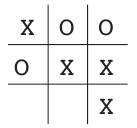
\includegraphics{02-introductionToRL/../assets/tic_tac_toe.jpeg}

Although the tic-tac-toe game is a simple problem, it cannot be
satisfactorily solved using classical techniques.

For instance, the classical ``\emph{minimax}'' solution from game theory
is not applicable here because it assumes the opponent's specific way of
playing. A \emph{minimax} player would never reach a game state from
which it could lose. Even if, in reality, it always won from that state
due to incorrect play by the opponent. The classical optimization
methods for sequential decision problems, like dynamic programming, can
find the best solution for any opponent. However, these methods need a
detailed description of the opponent as input, including the
probabilities of the opponent's moves in each board state.

Alternatively, this information can be estimated through experience,
such as playing numerous games against the opponent. The best approach
to this problem is to first learn a model of the opponent's behavior
with a certain level of confidence, and then use dynamic programming to
calculate an optimal solution based on the approximate opponent model.

Sutton and Barto (see pp.~9-12 Sutton and Barto 2018) propose the
following way to approach tic tac toe with Reinforcement Learning:

\section*{Setup:}\label{setup}
\addcontentsline{toc}{section}{Setup:}

\markright{Setup:}

\begin{itemize}
\item
  First we would set up a table of numbers (or labels), one for each
  possible state of the game.
\item
  Each number will be the latest estimate of the probability of our
  winning from that state.
\item
  We treat this estimate as the state's value, and the whole table is
  the learned value function.
\item
  State \(A\) has higher value than state \(B\), or is considered
  `better' than state \(B\), if the current estimate of the probability
  of our winning from \(A\) is higher than it is from \(B\).
\item
  If we always play \(Xs\), then for all states with three \(Xs\) in a
  row the probability of winning is 1, because we have already won.
\item
  Similarly, for all states with three \(Os\) in a row, or that are
  filled up, the correct probability is 0--we cannot win from them.
\item
  We set the initial values of all the other states to \(0.5\),
  representing a guess that we have a 50\% chance of winning.
\end{itemize}

\section*{Training:}\label{training}
\addcontentsline{toc}{section}{Training:}

\markright{Training:}

We then play many games against the opponent.

To select our moves we examine the states that would result from each of
our possible moves (one for each blank space on the board) and look up
their current values in the table. Most of the time we move
greedily,selecting the move that leads to the state with greatest value,
that is, with the highest estimated probability of winning.

Occasionally, however, we select randomly from among the other moves
instead. These are called exploratory moves because they cause us to
experience states that we might otherwise never see.

A sequence of moves made and considered during a game can be diagrammed
as the following figure:

\begin{figure*}

\centering{

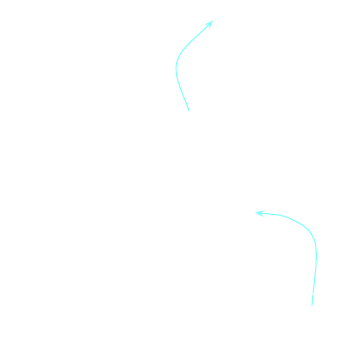
\includegraphics{02-introductionToRL/../assets/ch_00/diagram_sequence_tictactoe_play.png}

}

\caption{\label{fig-tic_tac_toc_diag}Figure taken from (Sutton and Barto
2018). A sequence of tic-tac-toe moves. Solid black lines represents
moves taken during a play. Dashed lines represent plausible but not
taken moves. The \(*\) symbol indicates the move currently estimated to
be the best. Thus the move \(e\) denotes an \emph{exploratory} move}

\end{figure*}%

\bookmarksetup{startatroot}

\chapter{Finite Markov Decision Processes
(MDPs)}\label{finite-markov-decision-processes-mdps}

That is what ChatGPT would answer to a 5-year-old kid. Alright, let's
imagine you have a little robot friend named Robo. Robo likes to explore
and do different things, but Robo doesn't always know what to do next. A
Markov Decision Process (MDP) is like giving Robo a set of rules to help
it decide what to do next based on where it is and what it knows.

Imagine Robo is in a room full of toys. Each toy is like a different
choice Robo can make, like playing with blocks or reading a book. But
Robo can't see the whole room at once, so it has to decide what to do
based on what it can see and remember.

In an MDP, Robo learns from its past experiences. If it finds that
playing with blocks usually makes it happy, it's more likely to choose
that again next time. But if it tries reading a book and doesn't like
it, it might choose something else next time.

So, a Markov Decision Process helps Robo make decisions by learning from
what it's done before and what it can see around it, kind of like how
you learn from playing with different toys and remembering which ones
you like best.

\section{The Agent--Environment
Interface}\label{the-agentenvironment-interface}

:::\{\#exm-roboClean\}

A mobile robot has the job of collecting empty soda cans in an office
environment. It has sensors for detecting cans, and an arm and gripper
that can pick them up and place them in an onboard bin; it runs on a
rechargeable battery. The robot's control system has components for
interpreting sensory information, for navigating, and for controlling
the arm and gripper. High-level decisions about how to search for cans
are made by a reinforcement learning agent based on the current charge
level of the battery. To make a simple example, we assume that only two
charge levels can be distinguished, comprising a small state set
\(\mathcal{S} = \{\texttt{high}, \texttt{low} \}\). In each state, the
agent can decide whether to

\begin{enumerate}
\def\labelenumi{\arabic{enumi}.}
\tightlist
\item
  actively \textbf{search} for a can for a certain period of time,
\item
  remain stationary and \textbf{wait} for someone to bring it a can, or
\item
  head back to its home base to \textbf{recharge} its battery.
\end{enumerate}

When the energy level is \textbf{high}, recharging would always be
foolis h, so we do not include it in the action set for this state. The
action sets are then
\(\mathcal{A}(\texttt{high}) = \{\texttt{search}, \texttt{wait}\}\) and
\(\mathcal{A}(\texttt{low}) = \{\texttt{search}, \texttt{wait}, \texttt{recharge}\}\).

The rewards are zero most of the time, but become positive when the
robot secures an empty can, or large and negative if the battery runs
all the way down. The best way to find cans is to actively search for
them, but this runs down the robot's battery, whereas waiting does not.
Whenever the robot is searching, the possibility exists that its battery
will become depleted. In this case the robot must shut down and wait to
be rescued (producing a low reward).

If the energy level is \textbf{high}, then a period of active search can
always be completed without risk of depleting the battery. A period of
searching that begins with a \textbf{high} energy level leaves the
energy level high \textbf{with} probability \(\alpha\) and reduces it to
low with probability \(1 - \alpha\). On the other hand, a period of
searching undertaken when the energy level is low leaves it low with
probability \(\beta\) and depletes the battery with probability
\(1 - \beta\). In the latter case, the robot must be rescued, and the
battery is then recharged back to \textbf{high}. Each can collected by
the robot counts as a unit reward, whereas a reward of \(-3\) results
whenever the robot has to be rescued. Let \(r_{\texttt{search}}\) and
\(r_{\texttt{wait}}\), with \(r_{\texttt{search}} > r_{\texttt{wait}}\),
denote the expected numbers of cans the robot will collect (and hence
the expected reward) while searching and while waiting respectively.
Finally, suppose that no cans can be collected during a run home for
recharging, and that no cans can be collected on a step in which the
battery is depleted. This system is then a finite MDP, and we can write
down the transition probabilities and the expected rewards, with
dynamics as indicated in the table on the left:

\begin{figure*}

\centering{

\captionsetup{labelsep=none}
\includegraphics{03-finiteMDPs/../assets/ch_03/recycling_robot_diagram.png}

}

\caption{\label{fig-robot-diagram}}

\end{figure*}%

\begin{exercise}[]\protect\hypertarget{exr-001}{}\label{exr-001}

Give a table analogous to that in (p.53, Ex. 3.3, Sutton and Barto
2018), but for \(p(s_0 , r |s, a)\). It should have columns for \(s\),
\(a\), \(s_0\) , \(r\), and \(p(s_0 , r |s, a)\), and a row for every
4-tuple for which \(p(s_0 , r |s, a) > 0\).

\end{exercise}

\section{Goals and Rewards}\label{goals-and-rewards}

\section{Returns and Episodes}\label{returns-and-episodes}

\section{Unified Notation for Episodic and Continuing
Tasks}\label{unified-notation-for-episodic-and-continuing-tasks}

\section{Policies and Value
Functions}\label{policies-and-value-functions}

\section{Optimal Policies and Optimal Value
Functions}\label{optimal-policies-and-optimal-value-functions}

\section{Optimality and
Approximation}\label{optimality-and-approximation}

\section{Summary}\label{summary}

\bookmarksetup{startatroot}

\chapter{Dynamic Programming}\label{dynamic-programming}

An explanation from ChatGPT. Alright, imagine you have a big puzzle to
solve, but it's too big for you to finish in one go. So, you decide to
break it into smaller puzzles, and you solve each of these small puzzles
one by one. But, here's the clever part: as you solve these small
puzzles, you remember the solutions. That way, if you come across the
same small puzzle again, you don't have to solve it all over again. You
already know the answer! Dynamic programming is like solving a big
puzzle by breaking it into smaller ones and remembering the solutions to
the smaller ones to make solving the big puzzle easier and faster.

\section{Policy Evaluation
(Prediction)}\label{policy-evaluation-prediction}

\section{Policy Improvement}\label{policy-improvement}

\section{Policy Iteration}\label{policy-iteration}

\section{Value Iteration}\label{value-iteration}

\section{Asynchronous Dynamic
Programming}\label{asynchronous-dynamic-programming}

\section{Generalized Policy
Iteration}\label{generalized-policy-iteration}

\section{Efficiency of Dynamic
Programming}\label{efficiency-of-dynamic-programming}

\section{Summary}\label{summary-1}

\bookmarksetup{startatroot}

\chapter{Applications}\label{applications}

\section{Recycling Robot}\label{recycling-robot}

\section{A robot with randomly moves in a grid
world.}\label{a-robot-with-randomly-moves-in-a-grid-world.}

\bookmarksetup{startatroot}

\chapter{Project proposal}\label{project-proposal}

\bookmarksetup{startatroot}

\chapter*{References}\label{references}
\addcontentsline{toc}{chapter}{References}

\markboth{References}{References}

\phantomsection\label{refs}
\begin{CSLReferences}{1}{0}
\bibitem[\citeproctext]{ref-Bertsekas2005}
Bertsekas, Dimitri P. 2005. \emph{Dynamic Programming and Optimal
Control. {V}ol. {I}}. Third. Athena Scientific, Belmont, MA.

\bibitem[\citeproctext]{ref-Bilgin2020}
Bilgin, E. 2020. \emph{Mastering Reinforcement Learning with Python:
Build Next-Generation, Self-Learning Models Using Reinforcement Learning
Techniques and Best Practices}. Packt Publishing.
\url{https://books.google.com.mx/books?id=s0MQEAAAQBAJ}.

\bibitem[\citeproctext]{ref-brandimarte2013numerical}
Brandimarte, Paolo. 2013. \emph{Numerical Methods in Finance and
Economics: A MATLAB-Based Introduction}. 2nd ed. Hoboken, New Jersey:
John Wiley \& Sons.

\bibitem[\citeproctext]{ref-Brunton2019}
Brunton, Steven L., and J. Nathan Kutz. 2019. \emph{Data-Driven Science
and Engineering}. Cambridge University Press, Cambridge.
\url{https://doi.org/10.1017/9781108380690}.

\bibitem[\citeproctext]{ref-Sutton2018}
Sutton, Richard S., and Andrew G. Barto. 2018. \emph{Reinforcement
Learning: An Introduction}. Second. Adaptive Computation and Machine
Learning. MIT Press, Cambridge, MA.

\bibitem[\citeproctext]{ref-Szepesvari2022}
Szepesvári, Csaba. 2022. \emph{Algorithms for Reinforcement Learning}.
Vol. 9. Synthesis Lectures on Artificial Intelligence and Machine
Learning. Springer, Cham.
\url{https://doi.org/10.1007/978-3-031-01551-9}.

\end{CSLReferences}

\bookmarksetup{startatroot}

\chapter*{List of Home Works and due
dates}\label{list-of-home-works-and-due-dates}
\addcontentsline{toc}{chapter}{List of Home Works and due dates}

\markboth{List of Home Works and due dates}{List of Home Works and due
dates}

\section*{Homework 001 due date: september 16,
2024-12:00:00}\label{homework-001-due-date-september-16-2024-120000}
\addcontentsline{toc}{section}{Homework 001 due date: september 16,
2024-12:00:00}

\markright{Homework 001 due date: september 16, 2024-12:00:00}

\begin{enumerate}
\def\labelenumi{\arabic{enumi}.}
\tightlist
\item
  Read (Sec 1.1, pp 1-2 Sutton and Barto 2018) and answer the following.
\end{enumerate}

Explain why Reinforcement Learning differs for supervised and
unsupervised learning.

\begin{enumerate}
\def\labelenumi{\arabic{enumi}.}
\setcounter{enumi}{1}
\item
  See the first Steve Brunton's youtube video about
  \href{https://www.youtube.com/watch?v=0MNVhXEX9to&list=PLMrJAkhIeNNQe1JXNvaFvURxGY4gE9k74}{Reinforcement
  Learning.} Then accordingly to its presentation explain what is the
  meaning of the following expression: \[
    V_{\pi}(s) = \mathbb{E}
   \left(
     \sum_{t} \gamma ^ {t} r_t | s_0 = s
   \right).
  \]
\item
  Form (Sec. 1.7 Sutton and Barto 2018) obtain a time line pear year
  from 1950 to 2012. Use the following format
  \href{https://kim.quarto.pub/milestones--bar-timelines/}{see
  https://kim.quarto.pub/milestones--bar-timelines/}
\end{enumerate}

\begin{Shaded}
\begin{Highlighting}[]
\FunctionTok{library}\NormalTok{(bibtex)}
\DocumentationTok{\#\# Activate the Core Packages}
\NormalTok{biblio }\OtherTok{\textless{}{-}}\NormalTok{ bibtex}\SpecialCharTok{::}\FunctionTok{read.bib}\NormalTok{(}\StringTok{"../references.bib"}\NormalTok{)}
\FunctionTok{library}\NormalTok{(tidyverse) }\DocumentationTok{\#\# Brings in a core of useful functions}
\end{Highlighting}
\end{Shaded}

\begin{verbatim}
-- Attaching core tidyverse packages ------------------------ tidyverse 2.0.0 --
v dplyr     1.1.4     v readr     2.1.5
v forcats   1.0.0     v stringr   1.5.1
v ggplot2   3.5.1     v tibble    3.2.1
v lubridate 1.9.3     v tidyr     1.3.1
v purrr     1.0.2     
-- Conflicts ------------------------------------------ tidyverse_conflicts() --
x dplyr::filter() masks stats::filter()
x dplyr::lag()    masks stats::lag()
i Use the conflicted package (<http://conflicted.r-lib.org/>) to force all conflicts to become errors
\end{verbatim}

\begin{Shaded}
\begin{Highlighting}[]
\FunctionTok{library}\NormalTok{(gt)        }\DocumentationTok{\#\# Tables}
\DocumentationTok{\#\# Specific packages}
\FunctionTok{library}\NormalTok{(milestones)}
\DocumentationTok{\#\# Initialize defaults}
\DocumentationTok{\#\# Initialize defaults}
\NormalTok{column }\OtherTok{\textless{}{-}} \FunctionTok{lolli\_styles}\NormalTok{()}

\NormalTok{data }\OtherTok{\textless{}{-}} \FunctionTok{read\_csv}\NormalTok{(}\AttributeTok{col\_names=}\ConstantTok{TRUE}\NormalTok{, }\AttributeTok{show\_col\_types=}\ConstantTok{FALSE}\NormalTok{, }\AttributeTok{file=}\StringTok{\textquotesingle{}rl\_time\_line.csv\textquotesingle{}}\NormalTok{)}

\DocumentationTok{\#\# Sort the table by date}
\NormalTok{data }\OtherTok{\textless{}{-}}\NormalTok{ data }\SpecialCharTok{|\textgreater{}}
  \FunctionTok{arrange}\NormalTok{(date)}

\DocumentationTok{\#\# Build a table}
\FunctionTok{gt}\NormalTok{(data) }\SpecialCharTok{|\textgreater{}}
  \CommentTok{\#cols\_hide(columns = event) |\textgreater{}}
  \FunctionTok{tab\_style}\NormalTok{(}\FunctionTok{cell\_text}\NormalTok{(}\AttributeTok{v\_align =} \StringTok{"top"}\NormalTok{),}
            \AttributeTok{locations =} \FunctionTok{cells\_body}\NormalTok{(}\AttributeTok{columns =}\NormalTok{ date)) }\SpecialCharTok{|\textgreater{}}
  \FunctionTok{tab\_source\_note}\NormalTok{(}\AttributeTok{source\_note =} \StringTok{"Source: Wikipedia"}\NormalTok{) }
\end{Highlighting}
\end{Shaded}

\begingroup
\fontsize{12.0pt}{14.4pt}\selectfont
\setlength{\LTpost}{0mm}
\begin{longtable*}{rll}
\toprule
date & event & Reference \\ 
\midrule\addlinespace[2.5pt]
{1957} & The term  “optimal control” appears & MR0090477 Bellman, Richard Dynamic programming. Princeton University Press, Princeton, NJ, 1957. xxv+342 pp. \\ 
{NA} & MDPs & MR0091859 Bellman, Richard A Markovian decision process.J. Math. Mech.6(1957), 679–684. \\ 
\bottomrule
\end{longtable*}
\begin{minipage}{\linewidth}
Source: Wikipedia\\
\end{minipage}
\endgroup

\begin{Shaded}
\begin{Highlighting}[]
\DocumentationTok{\#\# Adjust some defaults}
\NormalTok{column}\SpecialCharTok{$}\NormalTok{color }\OtherTok{\textless{}{-}} \StringTok{"orange"}
\NormalTok{column}\SpecialCharTok{$}\NormalTok{size  }\OtherTok{\textless{}{-}} \DecValTok{15}
\NormalTok{column}\SpecialCharTok{$}\NormalTok{source\_info }\OtherTok{\textless{}{-}} \StringTok{"Source: Wikipedia"}

\DocumentationTok{\#\# Milestones timeline}
\FunctionTok{milestones}\NormalTok{(}\AttributeTok{datatable =}\NormalTok{ data, }\AttributeTok{styles =}\NormalTok{ column)}
\end{Highlighting}
\end{Shaded}

\begin{verbatim}
Warning: Removed 1 row containing missing values or values outside the scale range
(`geom_text()`).
\end{verbatim}

\begin{verbatim}
Warning: Removed 1 row containing missing values or values outside the scale range
(`geom_segment()`).
\end{verbatim}

\begin{verbatim}
Warning: Removed 1 row containing missing values or values outside the scale range
(`geom_point()`).
\end{verbatim}

\begin{verbatim}
Warning: Removed 2 rows containing missing values or values outside the scale range
(`geom_segment()`).
\end{verbatim}

\begin{verbatim}
Warning in grid.Call.graphics(C_text, as.graphicsAnnot(x$label), x$x, x$y, :
conversion failure on 'The term “optimal control” appears' in 'mbcsToSbcs': dot
substituted for <e2>
\end{verbatim}

\begin{verbatim}
Warning in grid.Call.graphics(C_text, as.graphicsAnnot(x$label), x$x, x$y, :
conversion failure on 'The term “optimal control” appears' in 'mbcsToSbcs': dot
substituted for <80>
\end{verbatim}

\begin{verbatim}
Warning in grid.Call.graphics(C_text, as.graphicsAnnot(x$label), x$x, x$y, :
conversion failure on 'The term “optimal control” appears' in 'mbcsToSbcs': dot
substituted for <9c>
\end{verbatim}

\begin{verbatim}
Warning in grid.Call.graphics(C_text, as.graphicsAnnot(x$label), x$x, x$y, :
conversion failure on 'The term “optimal control” appears' in 'mbcsToSbcs': dot
substituted for <e2>
\end{verbatim}

\begin{verbatim}
Warning in grid.Call.graphics(C_text, as.graphicsAnnot(x$label), x$x, x$y, :
conversion failure on 'The term “optimal control” appears' in 'mbcsToSbcs': dot
substituted for <80>
\end{verbatim}

\begin{verbatim}
Warning in grid.Call.graphics(C_text, as.graphicsAnnot(x$label), x$x, x$y, :
conversion failure on 'The term “optimal control” appears' in 'mbcsToSbcs': dot
substituted for <9d>
\end{verbatim}

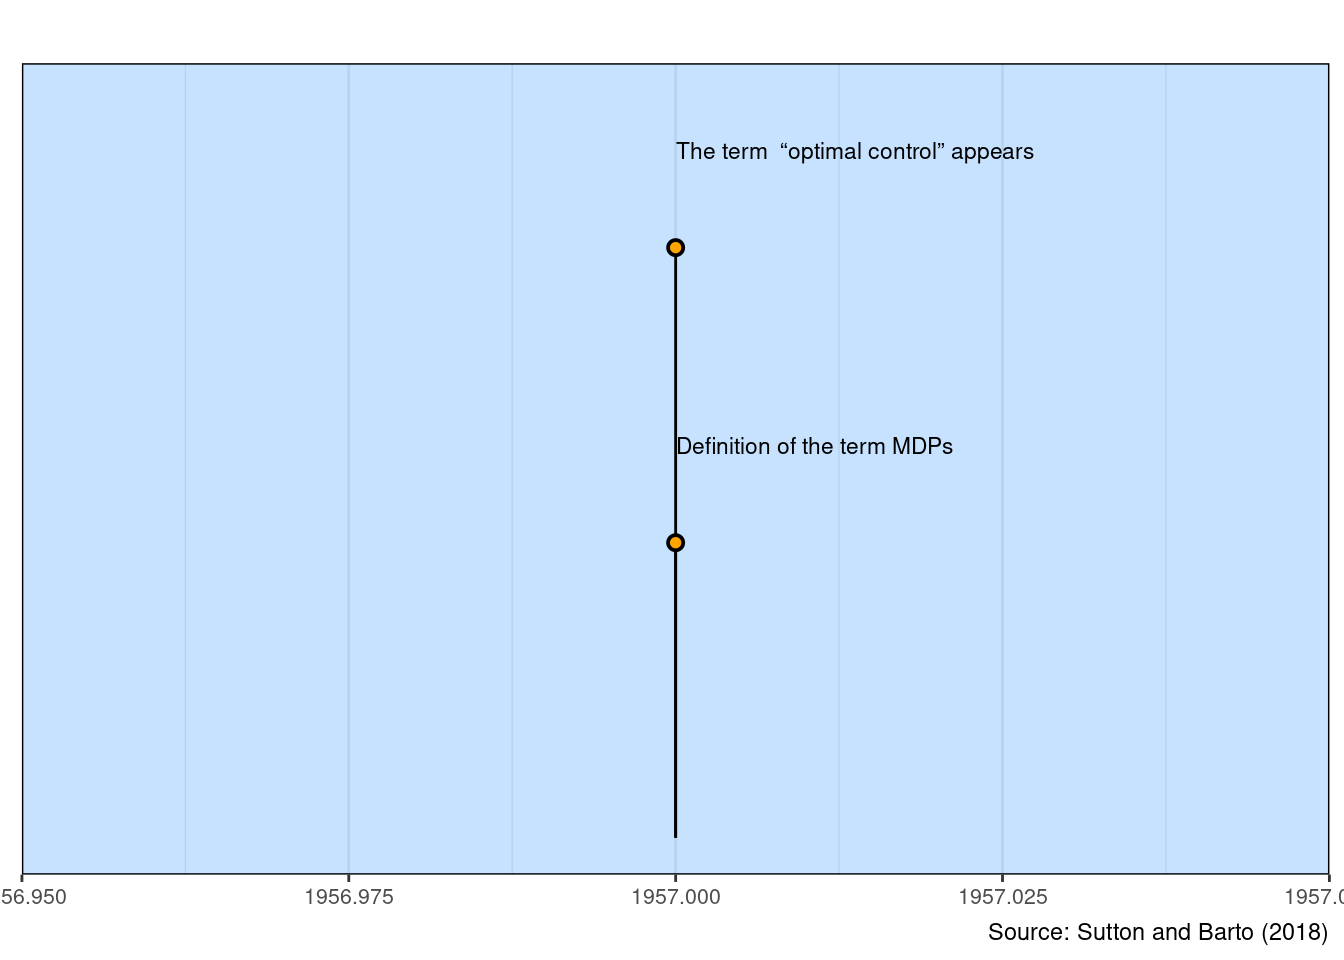
\includegraphics{homeworks/home_works_list_files/figure-pdf/unnamed-chunk-2-1.pdf}



\end{document}
